%/*******************************************************************************
% * Copyright (c) 2007, G. Weirich
% * All rights reserved. This program may not be distributed
% * or modified without prior written consent
% *
% * Contributors:
% *    G. Weirich - initial implementation
% *
% *  $Id: anleitung.tex 291 2007-10-09 04:25:28Z Gerry $
% *******************************************************************************/

\documentclass[a4paper]{scrartcl}
\usepackage{german}
\usepackage[utf8]{inputenc}
\usepackage{makeidx}
\usepackage{wrapfig}
\makeindex
% Hier ein etwas skurriler Block, der dazu dient, die Unterschiede
% zwischen pdflatex und latex auszubügeln
% Grafiken müssen als png oder gif (für pdflatex) und als eps (für Latex)
% vorhanden sein. Die Endung kann man beim \includegraphics jeweils weglassen,
% das System nimmt je nach Renderer die geeignete Variante.

\usepackage[pdftex]{graphicx}
\DeclareGraphicsExtensions{.pdf,.jpg,.png}

\usepackage{floatflt}
\usepackage[]{hyperref}
\usepackage{color}
\title{Elexis-Mythic}
\author{Gerry Weirich}

\begin{document}
\maketitle
\section{Einführung}
Dieses Plugin dient dazu, das Hämatologie-Laborgerät 'Mythic 18'\footnote{In der Schweiz von der Firma Polymed vertrieben} an Elexis anzubinden. Mit diesem Plugin können die vom Mythic gemessenen Laborparameter direkt in die Elexis-Datenbank eingelesen werden.

\subsection{Voraussetzungen}
Dieses Plugin benötigt Elexis 1.2.1 oder höher sowie ein Mythic Gerät. Ausserdem wird ein PC mit mindestens einer freien seriellen Schnittstelle und ein korrekt gepoltes serielles Kabel zur Verbindung des Mythic mit dem PC benötigt.

\section{Installation und Konfiguration}
Installieren Sie auf dem im Labor befindlichen PC das Plugin wie gewohnt. Verbinden Sie dann bei \textbf{ausgeschalteten} Geräten das Mythic mit der einem seriellen Port des Computers. Schalten Sie die serielle Datenübertragung am Mythic Gerät ein, falls noch nicht geschehen. (Vgl. Ihr Handbuch zum Mythic). Wählen Sie 9600,8,n,1 als Schnittstellenparameter.

Starten Sie dann Elexis und gehen Sie dort zu \textsc{Datei-Einstellungen-Datenaustausch-Mythic} (S. Abb. \ref{fig:mythic1}).
\begin{figure}[h]
    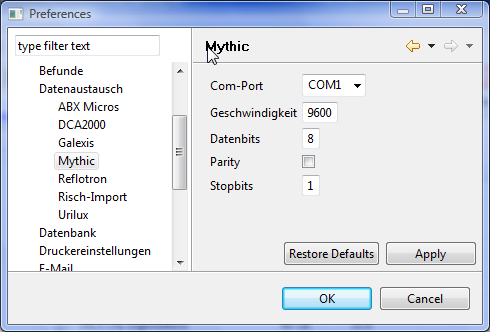
\includegraphics{mythic2}
    \caption{Einstellungen Mythic}
    \label{fig:mythic1}
\end{figure}
Hier stellen Sie den gewählten seriellen Port ein und die Schnittstellenparameter ein.


\section{Verwendung}
\begin{figure}[h]
\centering
    
\includegraphics{mythic1}
    \caption{Mythic einlesen}
    \label{fig:mythic2}
\end{figure}
Wenn das Plugin korrekt installiert ist, erscheint in der Labor-View automatisch ein neuer Button 'Mythic' (Abb. \ref{fig:mythic2}. Klicken Sie auf diesem Knopf, dann erscheint zunächst eine Dialogbox, in der Sie eingeben müssen, welchem Patienten die nächsten Resultate zugeordnet werden sollen. Danach wird die Verbindung hergestellt. Die Verbindung bleibt bestehen (Der Knopf erscheint eingerastet), bis entweder die Daten empfangen worden sind, oder 5 Minuten verstrichen sind, ohne dass Daten übertragen wurden, oder Sie den Knopf wieder manuell auslösen.

\medskip

Wichtig: In der aktuellen Version muss das Senden vom Mythic zum PC manuell ausgelöst werden (Resultate-$>$Optionen-$>$Send)

\pagebreak

\section{Kabelspezifikation}

\begin{figure}[htbp]
	\centering
		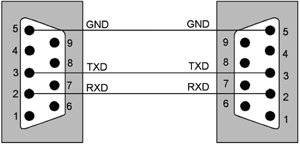
\includegraphics{kabel}
	\caption{Mythic Kabelkonfiguration}
	\label{fig:kabel}
\end{figure}

Es wird ein gerades, serielles Kabel ben\"otigt (gem\"ass Abb. \ref{fig:kabel})). Das Kabel muss an beiden Enden einen 9-poligen Stecker (1x weiblich und 1x m\"annlich) aufweisen.

\end{document}